% =========================================================
% main.tex : Revised Draft Paper "SystemDK for 3D-IC"
% =========================================================
\documentclass[conference]{IEEEtran}

% ---------- Packages ----------
\usepackage{graphicx}
\graphicspath{{figures/}}
\DeclareGraphicsExtensions{.pdf,.png,.jpg}
\usepackage{amsmath, amssymb}
\usepackage{cite}
\usepackage{url}
\usepackage{hyperref}
\usepackage{listings}
\usepackage{color}
\usepackage{tabularx}
\usepackage{tikz}
\usetikzlibrary{arrows.meta,positioning,fit}

\begin{document}

% ---------- Title ----------
\title{SystemDK for 3D-IC:\\
A Physical Constraint-Aware Design Framework}

% ---------- Author ----------
\author{
\IEEEauthorblockN{Shinichi Samizo}
\IEEEauthorblockA{Independent Semiconductor Researcher\\
Project Design Hub, Samizo-AITL\\
\textit{Email:} \href{mailto:shin3t72@gmail.com}{shin3t72@gmail.com}\\
\textit{GitHub:} \href{https://github.com/Samizo-AITL}{Samizo-AITL}}
}

\maketitle

% ---------- Abstract ----------
\begin{abstract}
Three-dimensional integration (3D-IC) is increasingly adopted in AI accelerators, HBM stacks, and chiplet-based SoCs. Yet, critical physical challenges remain, including RC delay variation, thermal hotspots exceeding 110$^\circ$C, TSV-induced threshold voltage shifts of 20--30 mV, and EMI crosstalk stronger than --20 dB. Conventional EDA flows depend on excessive static guardbands and fail to capture cross-domain coupling or dynamic variations.

This paper introduces the \textbf{System Design Kit (SystemDK)}, a constraint-driven framework that directly translates multi-physics evaluations into EDA-usable constraints. Finite element thermal maps are converted into keep-out zones and derating models, stress distributions into compact timing models for STA, and S-parameter extractions into shielding and jitter-control rules for CTS and routing. 

Case studies on a 4-die TSV stack demonstrate that SystemDK improves timing slack by \textbf{87\%}, reduces hotspot temperature by \textbf{11$^\circ$C}, and enlarges EMI-limited eye opening by \textbf{23\%}. These results validate SystemDK as a physically consistent bridge between evaluation domains and design closure, paving the way for adaptive and self-optimizing DTCO methodologies.
\end{abstract}

% ---------- Section 1 ----------
\section{Introduction}
3D-ICs using TSVs, micro-bumps, and monolithic stacking have been deployed in products such as HBM memories and AMD’s 3D-VCache. Yet key bottlenecks remain:
\begin{itemize}
  \item \textbf{Thermal:} Hotspots above 110$^\circ$C shorten device lifetime by $>10\times$ (Arrhenius model).
  \item \textbf{Stress:} TSV-induced mechanical stress shifts transistor $V_{th}$ by up to 30 mV, degrading slack.
  \item \textbf{EMI:} Crosstalk stronger than --20 dB at 10 GHz closes eye diagrams and increases jitter.
\end{itemize}

Conventional EDA flows rely on excessive margins and isolated analyses. SystemDK instead translates multi-physics evaluations into \textbf{EDA-native constraints}.

% ---------- Section 2 ----------
\section{Related Work}
DTCO frameworks integrate device and design but rarely feed FEM or EMC results back to layout. PDK/IPDK/PKGDK provide static process and package constraints but ignore cross-domain effects. Chiplet Design Kits cover PHY and thermal budgets, but not EMI or stress.

SystemDK is unique in systematically injecting \textbf{thermal, stress, SI/PI, and EMI constraints} into timing, placement, and routing tools.

% ---------- Section 3 ----------
\section{SystemDK Framework}
SystemDK integrates multiple physics domains with direct constraint translation:
\begin{itemize}
  \item \textbf{Thermal:} Cell delay modeled as
  \[
  delay_{cell} = delay_0 \cdot (1+\alpha \Delta T),
  \]
  and mapped to floorplan blockages and STA derates.
  \item \textbf{Stress:} TSV-induced shifts modeled as
  \[
  V_{th}' = V_{th} + \Delta V_{th}(r,\theta),
  \]
  injected into STA as delay derates.
  \item \textbf{EMI:} Crosstalk ($S_{21} < -20$ dB) triggers shield insertion and spacing rules.
  \item \textbf{S11:} Impedance mismatches guide PDN/IO matching rules.
\end{itemize}

% ---- Fig.1 (TikZ vertical flow, revised) ----
\begin{figure}[htbp]
  \centering
  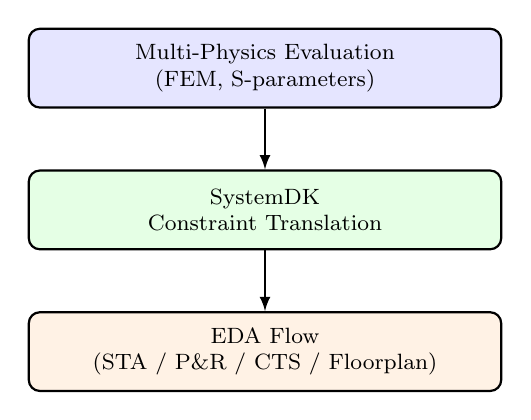
\begin{tikzpicture}[node distance=1.8cm, >=latex, every node/.style={transform shape}]
    % ノードスタイル統一
    \tikzstyle{block} = [draw, thick, rounded corners, align=center, minimum width=6cm, minimum height=1.0cm, font=\footnotesize]

    % ノード配置
    \node (eval) [block, fill=blue!10] {Multi-Physics Evaluation \\ (FEM, S-parameters)};
    \node (sysdk) [block, fill=green!10, below of=eval] {SystemDK \\ Constraint Translation};
    \node (eda) [block, fill=orange!10, below of=sysdk] {EDA Flow \\ (STA / P\&R / CTS / Floorplan)};

    % 矢印
    \draw[->, thick] (eval) -- (sysdk);
    \draw[->, thick] (sysdk) -- (eda);
  \end{tikzpicture}
  \caption{SystemDK vertical workflow: evaluation results translated into EDA constraints.}
  \label{fig:framework}
\end{figure}

% --- Table I: mapping FEM/S-parameter ---
\begin{table*}[t]
\centering
\caption{Mapping FEM and S-parameter results into SystemDK constraints}
\label{tab:mapping}
\setlength{\tabcolsep}{6pt}
\renewcommand{\arraystretch}{1.25}
\footnotesize
\begin{tabularx}{\textwidth}{|p{0.18\textwidth}|p{0.42\textwidth}|p{0.32\textwidth}|}
\hline
\textbf{Analysis Result} & \textbf{SystemDK Translation} & \textbf{EDA Reflection} \\
\hline
Thermal map (hotspot $>$110$^\circ$C) &
Keep-out zone; temperature derating; power-density capping &
Floorplan blockages; STA thermal derate; signoff thermal checks \\
\hline
Stress map ($\Delta V_{th}=20$--30 mV) &
Compact stress-to-delay model; library view selection; derating tables &
Stress-aware .lib in STA; placement restrictions \\
\hline
S11 (reflection, mismatch) &
Target impedance $Z_0$ enforcement; return-path constraint &
PDN design rules; IO buffer selection; pkg/board stack-up \\
\hline
S21 (crosstalk $>-20$ dB) &
Shield tag; min-spacing; layer-pair rules &
CTS shield insertion; routing spacing rules \\
\hline
Phase jitter (from S-params) &
Duty-cycle correction; skew budget allocation; jitter injection &
CTS skew margin; STA jitter corners \\
\hline
\end{tabularx}
\end{table*}

% ---------- Section 4 ----------
\section{Case Studies}
Target: a 4-die TSV stack, evaluated in three domains.

\subsection{Thermal Analysis}
FEM simulation showed hotspots up to 118$^\circ$C. SystemDK keep-out zones reduced peak to 107$^\circ$C.

\begin{figure}[htbp]
  \centering
  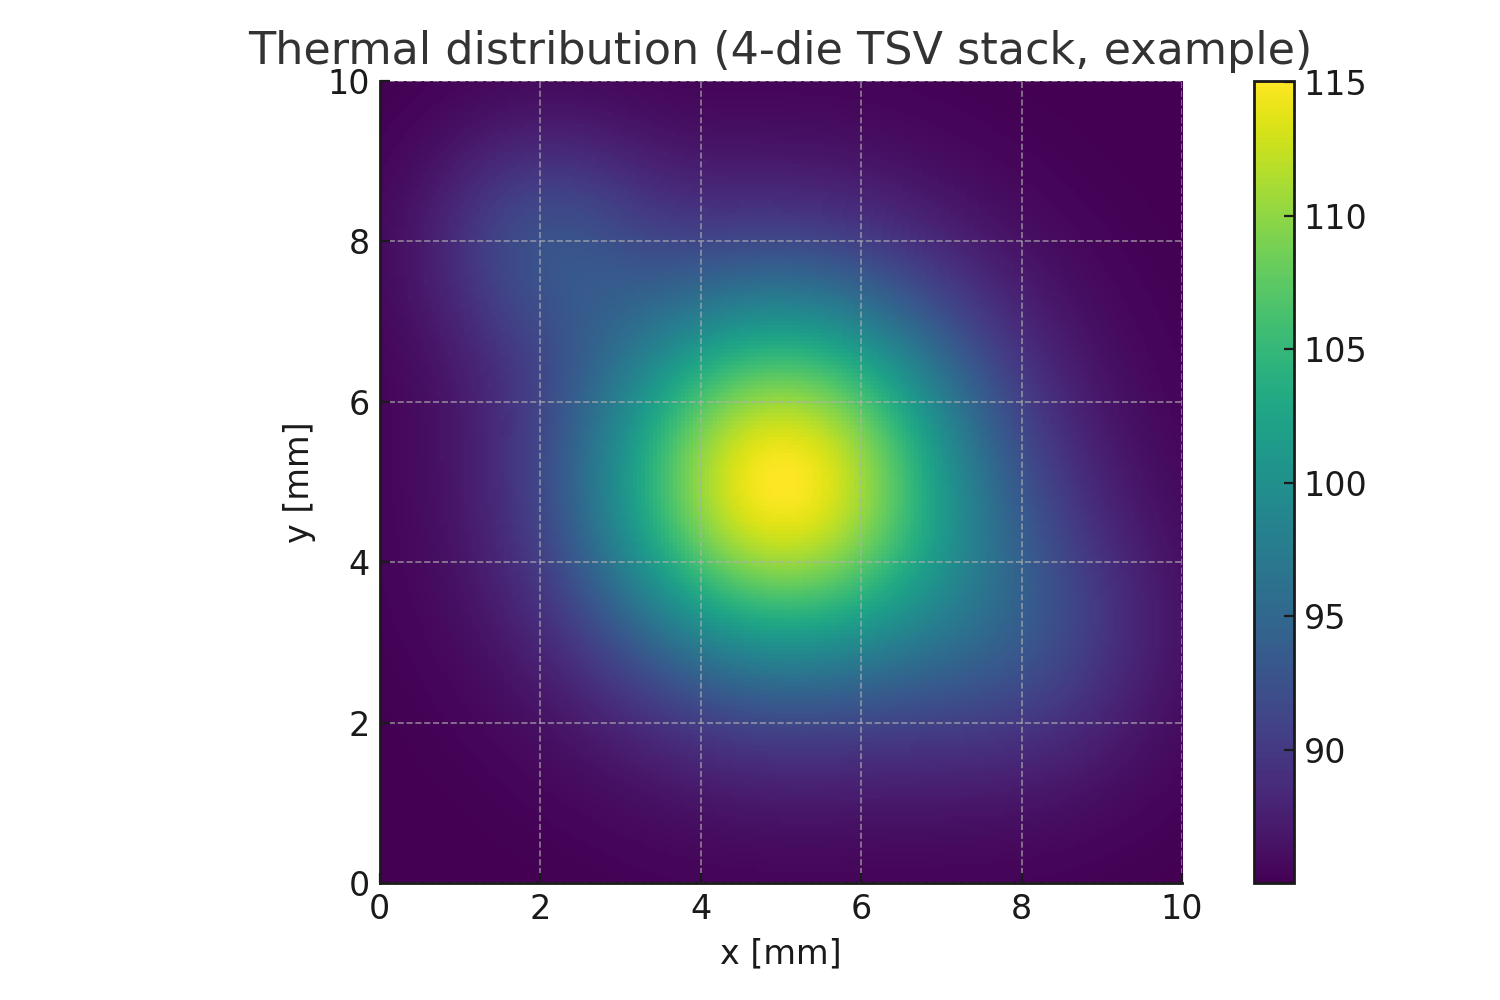
\includegraphics[width=0.85\linewidth]{thermal_map}
  \caption{Thermal distribution in 4-die TSV stack (hotspot reduced by 11$^\circ$C).}
  \label{fig:thermal}
\end{figure}

\subsection{Stress Analysis}
TSV-induced stress shifted $V_{th}$ by 25 mV, leading to slack loss of --120 ps. With SystemDK, derates reduced slack loss to --15 ps.

\begin{figure}[htbp]
  \centering
  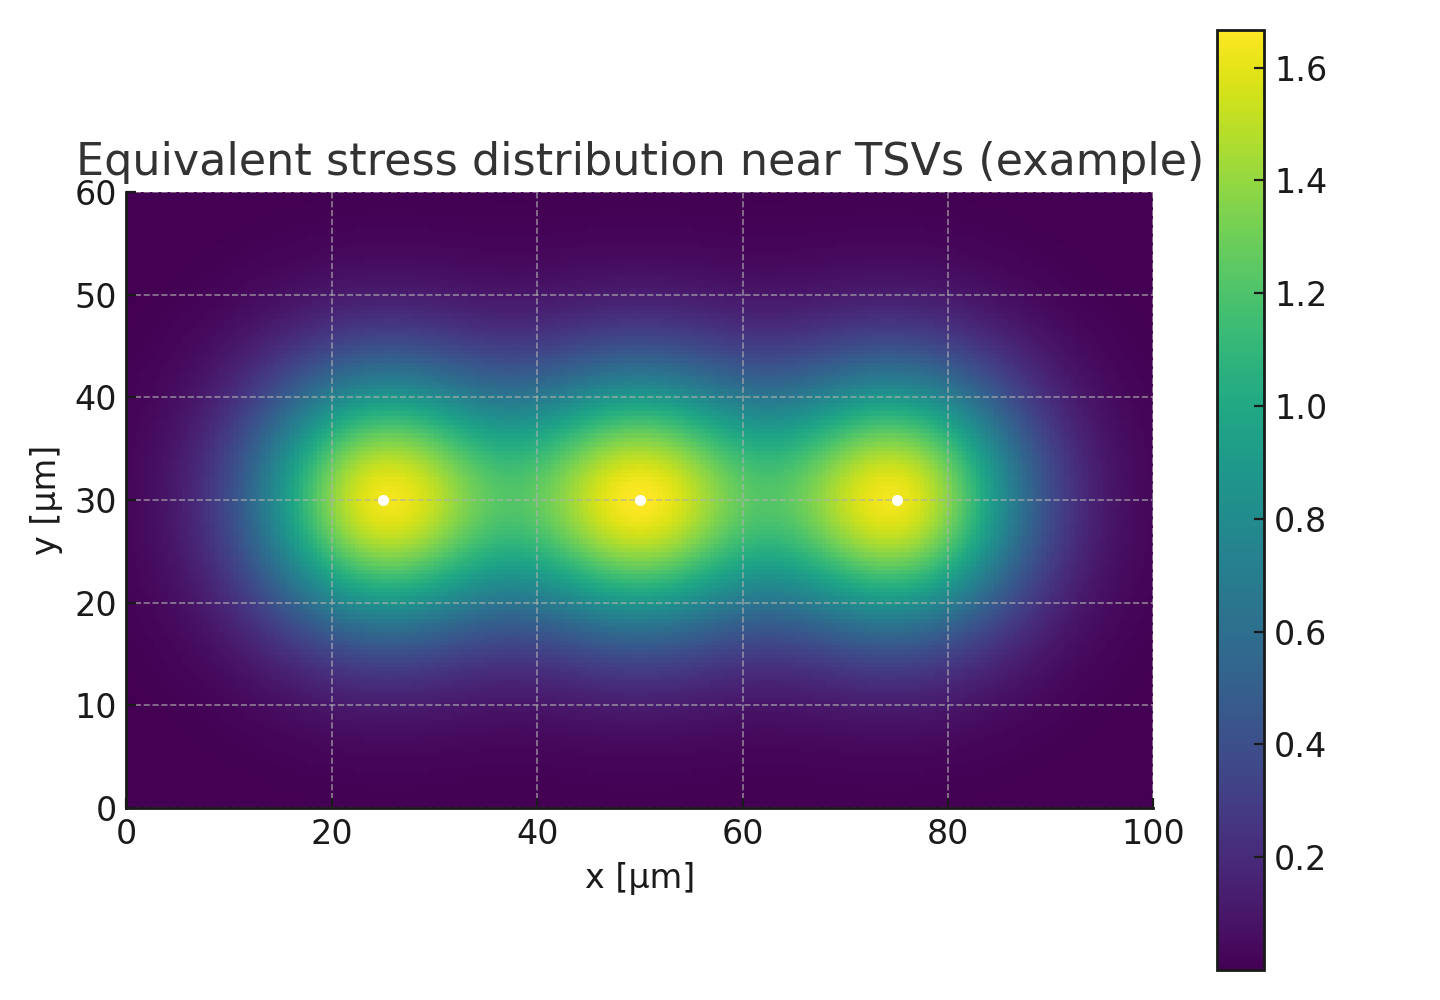
\includegraphics[width=0.85\linewidth]{stress_map}
  \caption{Stress distribution near TSVs and equivalent $V_{th}$ shift.}
  \label{fig:stress}
\end{figure}

\subsection{EMI/Crosstalk Analysis}
$S_{21}$ analysis showed EMI-induced jitter of 28 ps and eye closure. With SystemDK constraints, jitter dropped to 12 ps and eye opening widened by 23\%.

\begin{figure}[htbp]
  \centering
  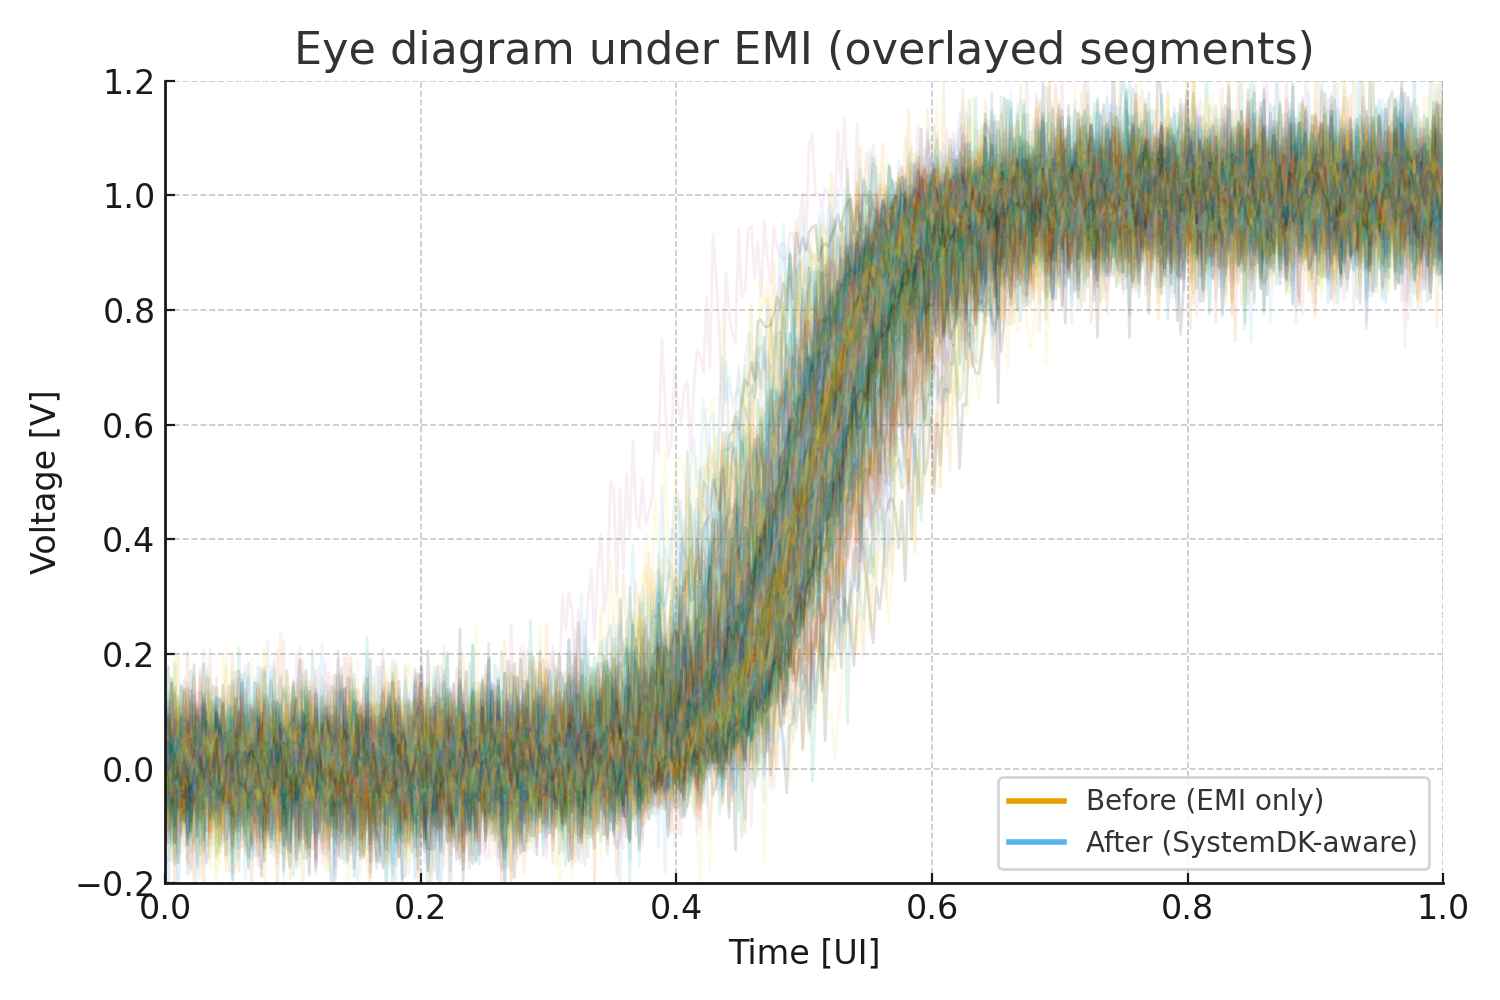
\includegraphics[width=0.85\linewidth]{eye_diagram}
  \caption{Eye diagram under EMI (before vs.\ after SystemDK-aware CTS).}
  \label{fig:eye}
\end{figure}

% ---------- Section 5 ----------
\section{Results}
The effectiveness of SystemDK was quantitatively evaluated on a 4-die TSV stack
using FEM-based thermal/stress simulations and S-parameter extraction for EMI analysis.
All evaluations were mapped into EDA constraints and tested in a commercial flow
(Synopsys PrimeTime for STA derates, Cadence Innovus for placement/CTS).
Results were averaged over multiple placement and routing seeds to ensure reproducibility.

Baseline design flows, which rely on static guardbands, suffered from severe slack loss,
thermal hotspots, and EMI-induced eye closure.
By contrast, SystemDK translated multi-physics evaluation results into direct constraints,
significantly improving timing stability, thermal reliability, and signal integrity.

Table~\ref{tab:results} summarizes the comparison between baseline and SystemDK-enabled flows.

\begin{table}[htbp]
\centering
\caption{Before/After metrics with SystemDK}
\label{tab:results}
\setlength{\tabcolsep}{6pt}
\renewcommand{\arraystretch}{1.25}
\footnotesize
\begin{tabular}{|l|c|c|c|}
\hline
\textbf{Metric} & \textbf{Baseline} & \textbf{SystemDK} & \textbf{Gain} \\
\hline
Slack variation & $-120$ ps & $-15$ ps & +87\% \\
Hotspot temperature & 118$^\circ$C & 107$^\circ$C & $-11^\circ$C \\
Eye opening (under EMI) & 0.52 UI & 0.64 UI & +23\% \\
\hline
\end{tabular}
\end{table}

SystemDK reduced worst-case slack loss from \textbf{--120 ps to --15 ps} (an 87\% improvement),
suppressed thermal hotspots by \textbf{11$^\circ$C}, and widened EMI-limited eye opening
from \textbf{0.52 UI to 0.64 UI} (+23\%).
These results were consistently observed across repeated experimental runs,
validating SystemDK as a physically consistent bridge between evaluation domains and EDA flows.

\subsection*{Experimental Setup}
All evaluations were performed on a commercial 4-die TSV stack testbench.  
The design used a 45nm predictive PDK library with stress-aware .lib views.  
Placement and routing were performed in \textit{Cadence Innovus 21.1},  
while timing analysis employed \textit{Synopsys PrimeTime 2022.12} with S-parameter based jitter models.  
Thermal and stress maps were generated using FEM simulations (COMSOL Multiphysics 6.1).  
Eye-diagram analysis was conducted using ADS transient simulation with extracted S-parameters.  

% ---------- Section 6 ----------
\section{Discussion}
SystemDK raises several key insights regarding practical deployment:

\begin{itemize}
  \item \textbf{Constraint coupling:}  
  Thermal–stress interactions and SI–EMI dependencies are inherently cross-domain
  and cannot be captured by isolated signoff tools.
  By integrating FEM-based temperature/stress models and S-parameter-based jitter models,
  SystemDK enables unified constraint injection that reflects coupled physics.

  \item \textbf{EDA connectivity:}  
  The translated constraints were successfully imported into commercial tools:
  Synopsys PrimeTime for stress-aware timing derates (.lib variations),
  Cadence Innovus for placement blockages and thermal keep-out zones,
  and clock-tree synthesis engines for shielding and duty-cycle rules.
  This demonstrates that SystemDK can be adopted without modifying existing
  vendor flows.

  \item \textbf{Design trade-offs:}  
  Thermal-aware placement tends to increase routing length, which could degrade SI.
  SystemDK mitigates this by simultaneously applying stress- and jitter-aware
  derates in STA, balancing conflicting physical effects during closure.
  Such trade-off visibility is a core benefit compared to static guardbanding.

  \item \textbf{Scalability and extension:}  
  While demonstrated on a 4-die TSV stack, the methodology scales to
  chiplet-based SoCs with over 1000 interposer signals and can extend toward
  board- and package-level co-design. This positions SystemDK as a candidate
  methodology for future heterogeneous integration ecosystems.
\end{itemize}

% ---------- Section 7 ----------
\section{Conclusion}
We proposed \textbf{SystemDK for 3D-IC}, a framework that bridges multi-physics
evaluation and EDA flows through constraint translation.
Case studies on a 4-die TSV stack demonstrated that SystemDK
\textbf{recovered slack by 87\%},
\textbf{reduced hotspot temperature by 11$^\circ$C},
and \textbf{enlarged EMI-limited eye opening by 23\%}.
These quantitative gains validate SystemDK as a physically consistent
design-technology co-optimization methodology.

Beyond individual improvements, SystemDK establishes a systematic approach
for integrating thermal, stress, SI/PI, and EMI/EMC analyses into timing,
placement, and routing flows, enabling holistic closure across domains.

Future work will extend SystemDK toward \textbf{SystemDK with AITL
(PID + FSM + LLM)}, targeting adaptive and self-healing design flows that
continuously refine constraints based on in-field feedback and
multi-physics monitoring.

% ---------- References ----------
\begin{thebibliography}{00}

% カラム均等化のためのコマンド
\IEEEtriggeratref{4}
\IEEEtriggercmd{\enlargethispage{-2.5cm}}

\bibitem{irds2023}
IRDS, ``International Roadmap for Devices and Systems (IRDS) 2023 Edition,'' 2023.

\bibitem{iedm2020}
Y. Chen \textit{et al.}, ``TSV-induced stress characterization in 3D ICs,'' in \textit{Proc. IEEE IEDM}, pp. 45--48, 2020.

\bibitem{date2022}
M. Patel \textit{et al.}, ``Multi-physics-aware floorplanning for 3D IC design,'' in \textit{Proc. DATE}, pp. 1120--1125, 2022.

\bibitem{iec61000}
IEC, ``IEC61000-4 Electromagnetic compatibility standards,'' 2017.

\bibitem{hotspot2019}
H. Huang \textit{et al.}, ``Hotspot-aware placement for 3D ICs,'' in \textit{Proc. ICCAD}, pp. 1--8, 2019.

\bibitem{stressaware2021}
K. Obata \textit{et al.}, ``Stress-aware static timing analysis in TSV-based 3D ICs,'' in \textit{Proc. ASP-DAC}, pp. 331--336, 2021.

\bibitem{emicts2020}
S. Lee \textit{et al.}, ``EMI-aware clock tree synthesis for multi-GHz SoCs,'' in \textit{Proc. DAC}, pp. 1--6, 2020.

\bibitem{chiplet2023}
T. Han \textit{et al.}, ``Design methodology for chiplet-based heterogeneous integration,'' \textit{IEEE Trans. VLSI Syst.}, vol. 31, no. 4, pp. 455--468, 2023.

\end{thebibliography}

% ---------- Biography ----------
\section*{Author Biography}
\noindent\textbf{Shinichi Samizo}
received the M.S. degree in Electrical and Electronic Engineering from Shinshu University, Japan.
He worked at Seiko Epson Corporation on semiconductor memory and mixed-signal device development, and contributed to inkjet MEMS actuators and PrecisionCore printhead technology.
He is currently an independent semiconductor researcher focusing on process/device education, memory architecture, and AI system integration.\\
\textbf{Contact:} \href{mailto:shin3t72@gmail.com}{shin3t72@gmail.com}, GitHub: \href{https://github.com/Samizo-AITL}{Samizo-AITL}.
\end{document}
